\chapter{ Results }


During this chapter we are going to show several results in order to answer the 
initial questions we had formulated initially such as, are BAO properties changing with the 
scale of the tracer halo population? 

The simulation Multidark Planck (MDPL) is going to be used throughout this chapter. It
belongs to the MultiDark database, uses a Planck cosmology (table \ref{plancktable}), has 
a box length of $L=1$Gpc/h and a number of particles equal to $3840^3$.
Specifically for this work, it was used a MDPL halo catalogue constructed with Friend of 
Friends algorithm and a linking length of 0.2 \footnote{ Data taken from \url{https://www.cosmosim.org/cms/simulations/MDPL/}}. From the complete halo catalog are selected different halo populations
depending on a halo mass range, five different halo populations are constructed as shown in table \ref{pophalos}.

\

The main objective for the construction of these populations is to find if there is 
a difference in the behavior of the correlation function of every population, 
and likewise the BAO that is recovered from the correlation function. 
In the figures \ref{pophalos}, the correlation function calculated for every population 
is shown. There are some differences, a first one is that the correlation function amplitude 
changes with the population, the more massive halo populations have a larger amplitude
compared with the lower ones, at least this is clear from the maximum value obtained in
each case. Other notorious difference is the decrease in the error bars shown for each
population as they become more massive. This effect appears due to the way the error is
calculated. 


\begin{table}
\begin{center}
  \begin{tabular}{ | c | c | c | }
    \hline \hline
    MDPL population & Mass range $M_{\odot}$& Number of halos \\ \hline \hline
    4 & $ M \geqslant 1e14$ & 32436 \\ \hline
    3 & $ 1e13 \leq M < 1e14 $ & 443356\\ \hline
    2 & $ 1e12 \leq M < 1e13$ & 3687677\\ \hline
    1 & $ 1e11 \leq M < 1e12$ & 32868688 \\ \hline
    0 & $ 1e10 \leq M < 1e11$ &  69822513 \\ \hline
  \end{tabular}  
   \caption{ Populations constructed from the mass range that appears in column two. }
\label{pophalos}
\end{center}
\end{table}

\begin{figure}[htbp]
   %\begin{center}
   $
    \begin{array}{ll}
    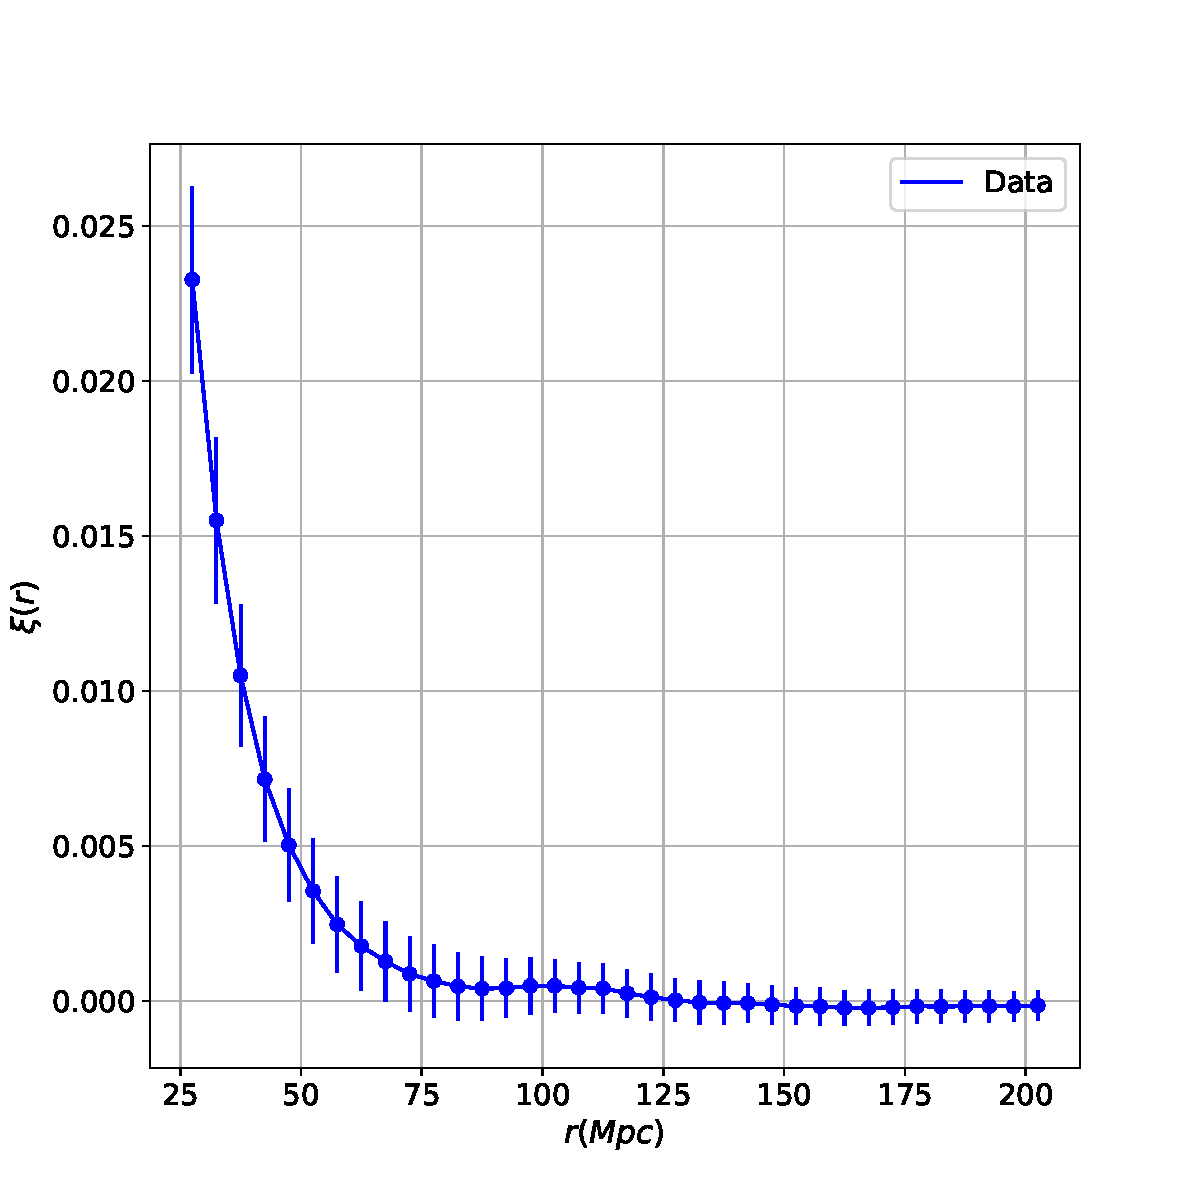
\includegraphics[width=85mm]{Images/chapter4/CF_all_1e11.pdf}&
    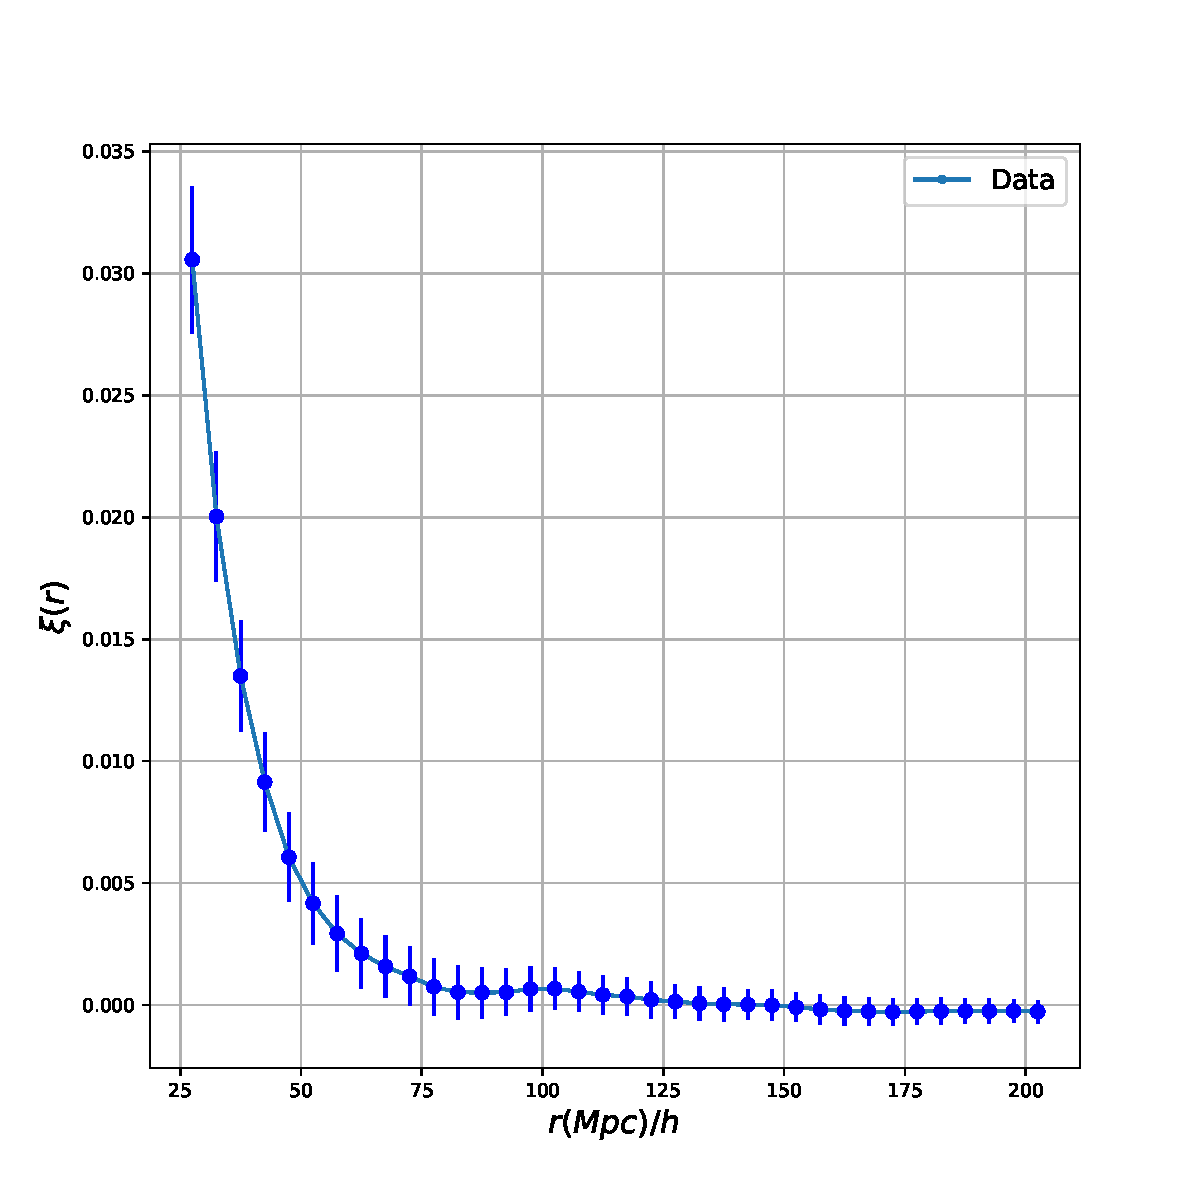
\includegraphics[width=85mm]{Images/chapter4/CF_all_1e12.pdf}\\
    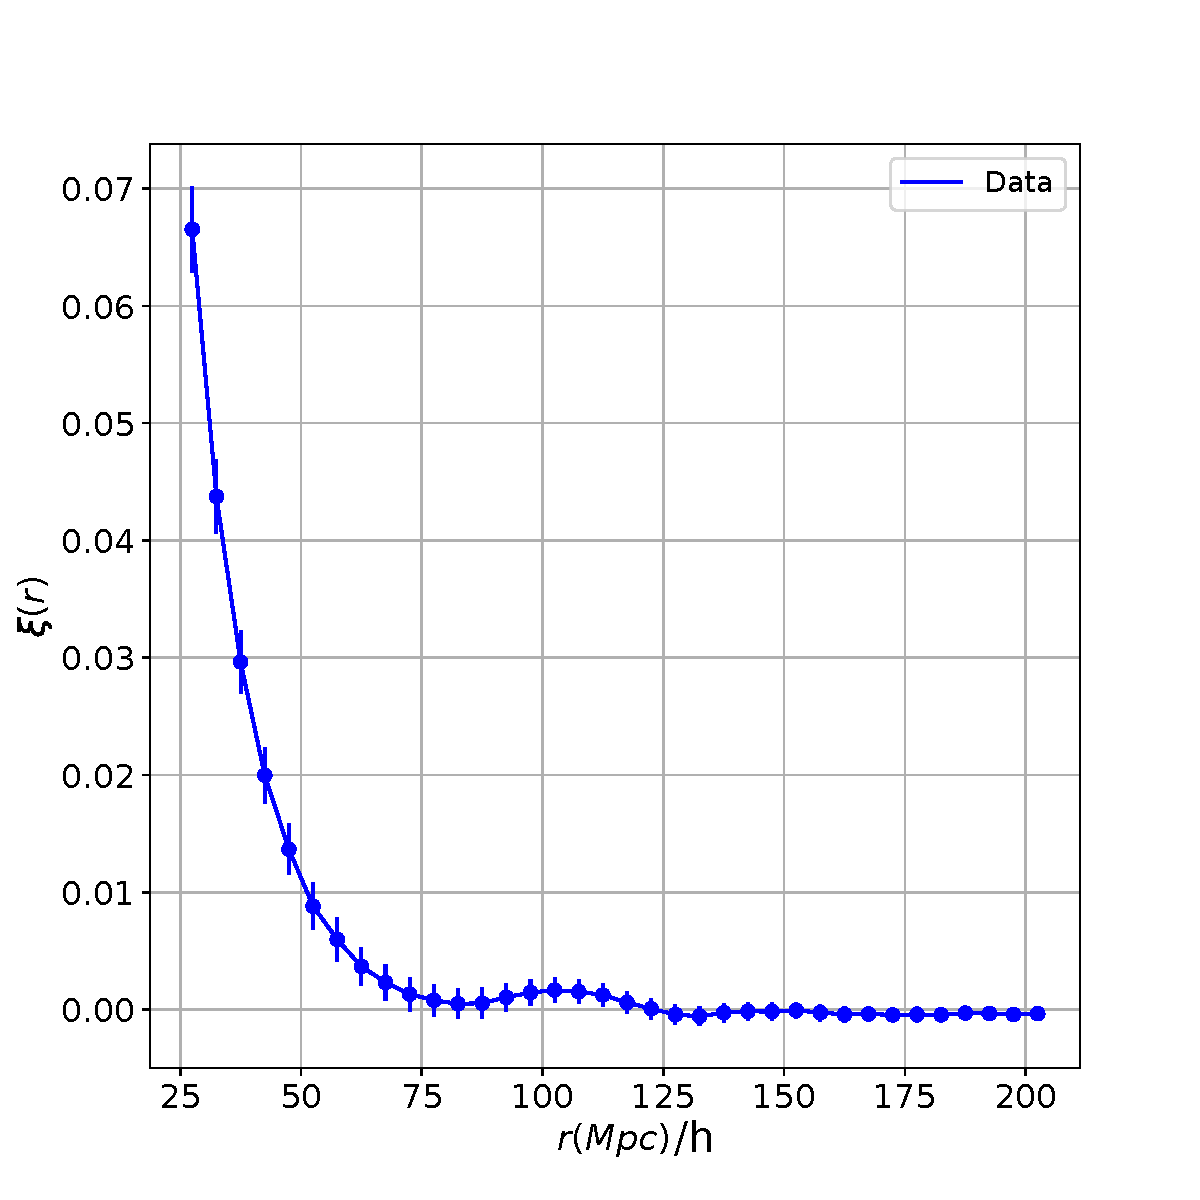
\includegraphics[width=85mm]{Images/chapter4/CF_all_1e13.pdf}&
    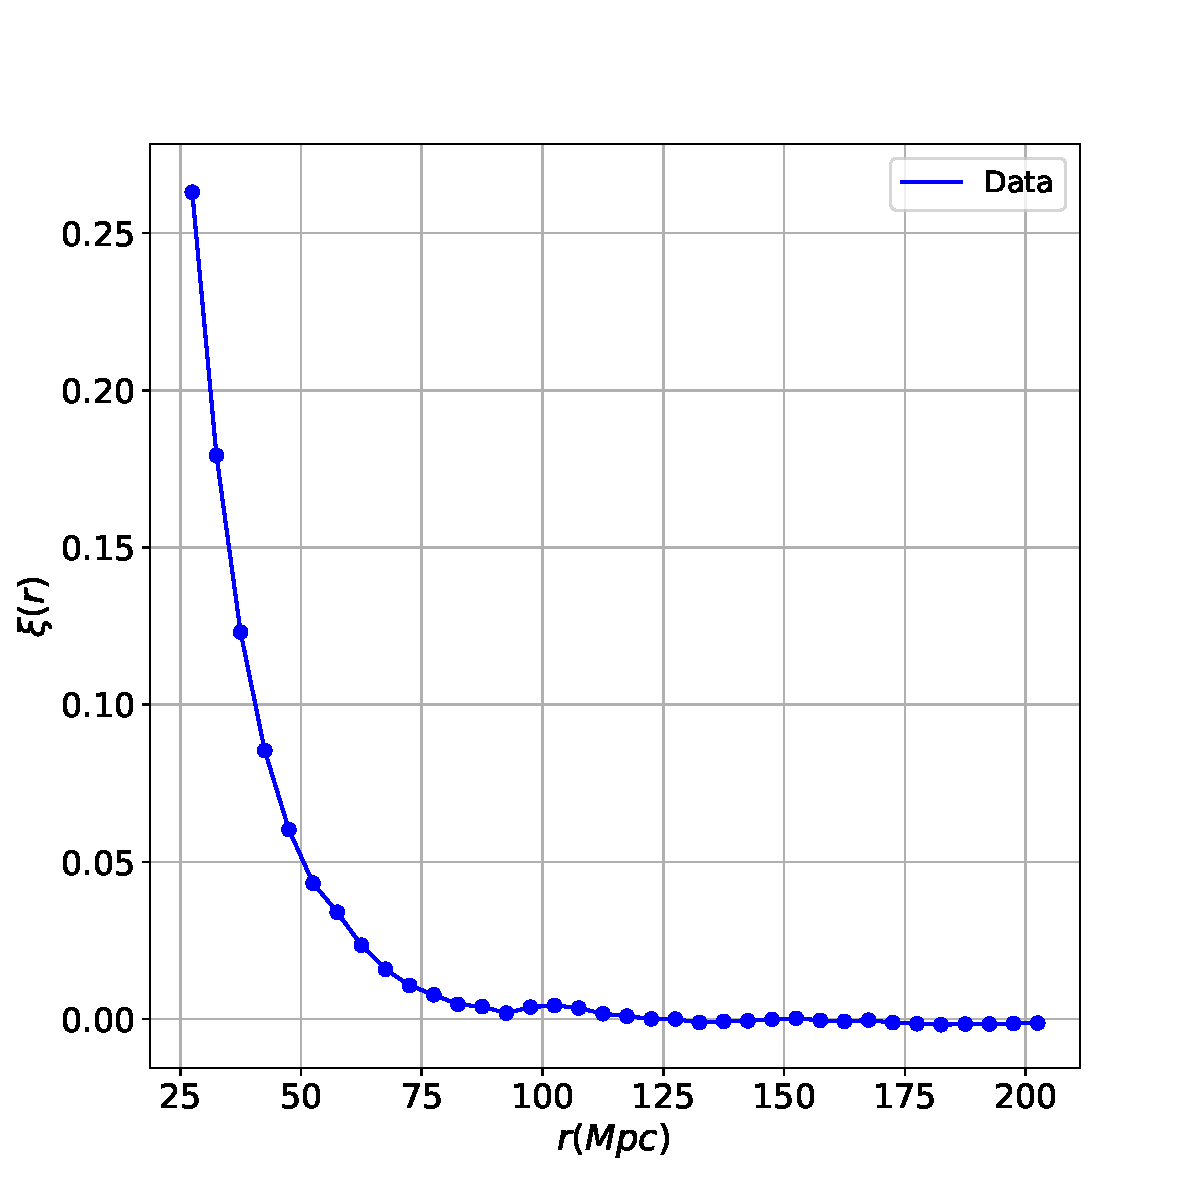
\includegraphics[width=85mm]{Images/chapter4/CF_all_1e14.pdf}
    \end{array}$
  %\end{center}
   \caption{The correlation functions for populations $1$, $2$, $3$ and $4$ are displayed from the upper left to the lower right. }
   \label{CFall}
\end{figure}

\section{ Correlation functions for MDPL populations}

\subsection{ Random Sampling and Number of particles}

\section{ Correlation function fit}

\subsection{ Correlation function of subsamples }

\section{Baryonic acoustic oscillations in the populations of MDPL }

As mentioned previously, the BAO peak is clearly detected for every population 
and the fit to the BAO signal was properly calculated using a Gaussian function. 
Let us see the situation in more detail. There are different populations, each of 
them have the following ranges in mass, the population $1$: $M \leq 1e11 M_{\odot}$, 
the population $2$: $ 1e11 M_{\odot} <M \leq 1e12 M_{\odot}$, the population $3$: $ 1e12 M_{\odot} <M \leq 1e13 M_{\odot}$ 
and finally the population $4$: $ 1e13 M_{\odot} <M \leq 1e14 M_{\odot}$. 
Thus, we are considering per population, more massive halos each time and that
way be able to analyze if there is an effect on the properties of BAO obtained
for each population. It is important to take into account that more massive halos 
trace higher density peaks in the matter density field which should lead, in principle, 
to a stronger correlation than the less massive ones, thus a better detection of 
the BAO signal. For example, in figure \ref{ampl} an increase of the amplitude 
of the BAO for more massive halos is obtained as precisely expected for a stronger
correlation. If the amplitude of the BAO for the population 1 is taken as reference
and using the percent error formula, the difference with the third and fourth 
population are $\approx 66.47\%$ and $\approx 90.82\%$, supporting the idea of the
increment in amplitude. 

Another important factor is the gravitational interaction among more massive halos.
Since larger masses exert greater gravitational attraction than smaller masses, 
the more massive halos should be closer among them, causing a smaller broadening
in the BAO peak compared with the less massive ones. This can be seen in the
figure \ref{width} where the width of the BAO decreases with more massive halos.
Again, taking the population 1 as reference it is obtained $\approx 18.54\%$ and
$\approx 65.38\%$ for the third and forth population respectively.

The position of the BAO depends on the sound horizon scale as shown in \ref{SH},
gravitational interactions causes a change in the BAO width \cite{Pilar} not in 
its position. But in the figure \ref{mean} a decrease in the BAO position with 
more massive halo population appears. But using the population $1$ as reference
the difference with the third and fourth population are $\approx 2.07\%$ and $\approx 3.9\%$,
is very small. Hence, it would not be a very reliable result. 
	

\begin{figure}[h]
   %\begin{center}
   $
    \begin{array}{lll}
    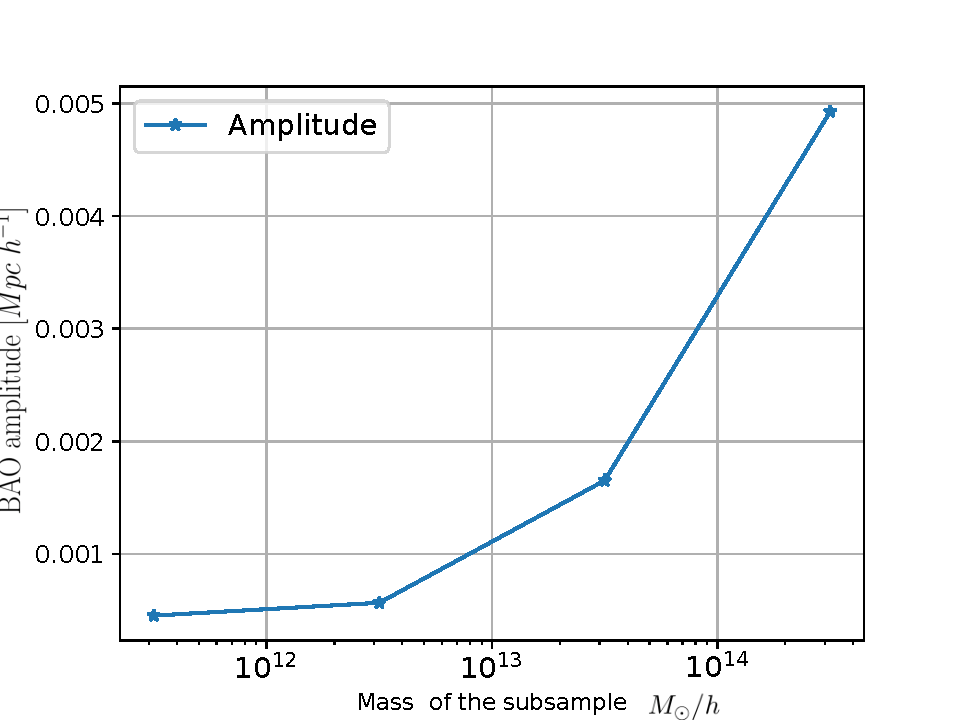
\includegraphics[width=55mm]{Images/chapter4/Amp_vs_Mh.pdf}&
    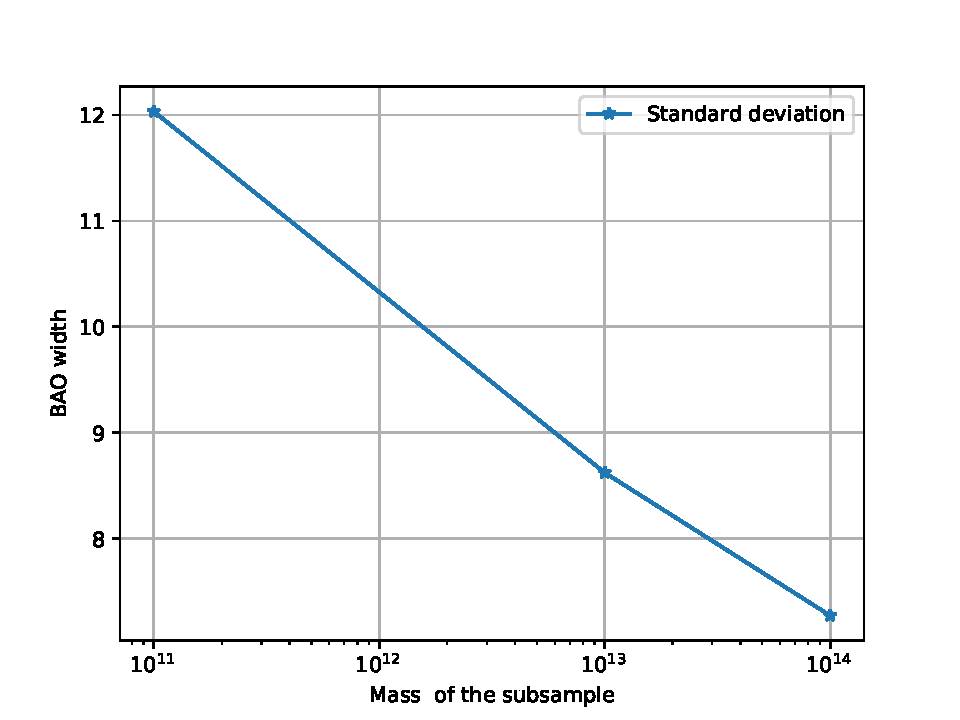
\includegraphics[width=55mm]{Images/chapter4/Width_vs_Mh.pdf}&
    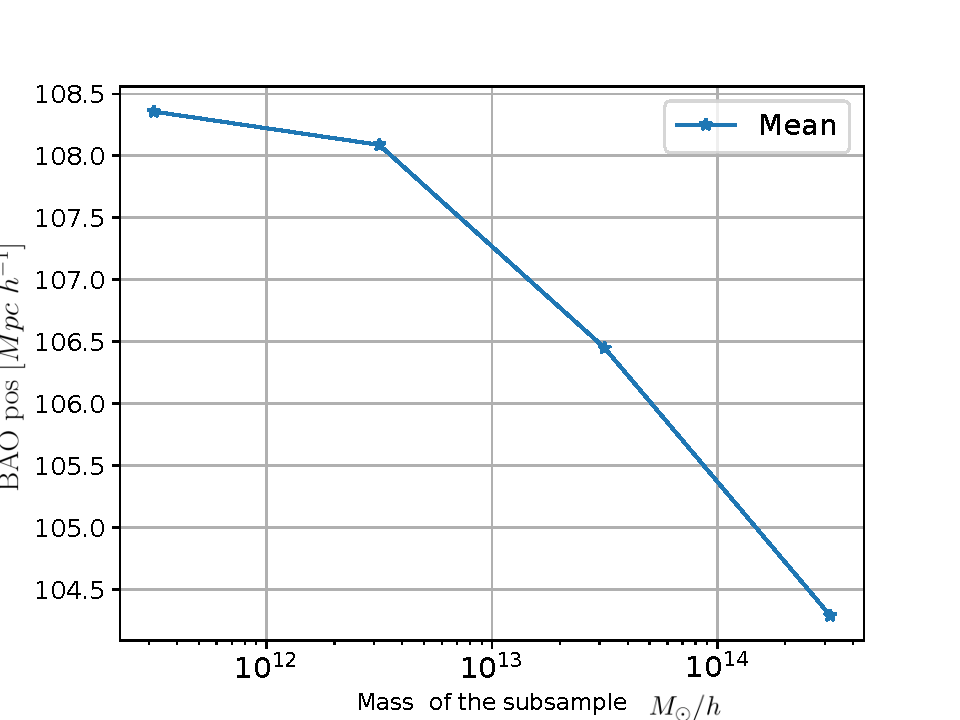
\includegraphics[width=55mm]{Images/chapter4/Pos_vs_Mh.pdf}
    \end{array}$
  %\end{center}
   \caption{Figure caption}
   \label{CFall}
\end{figure}
	


\begin{comment}
%**********************************************************************************************************************
\begin{figure}[htbp]
       \centering
               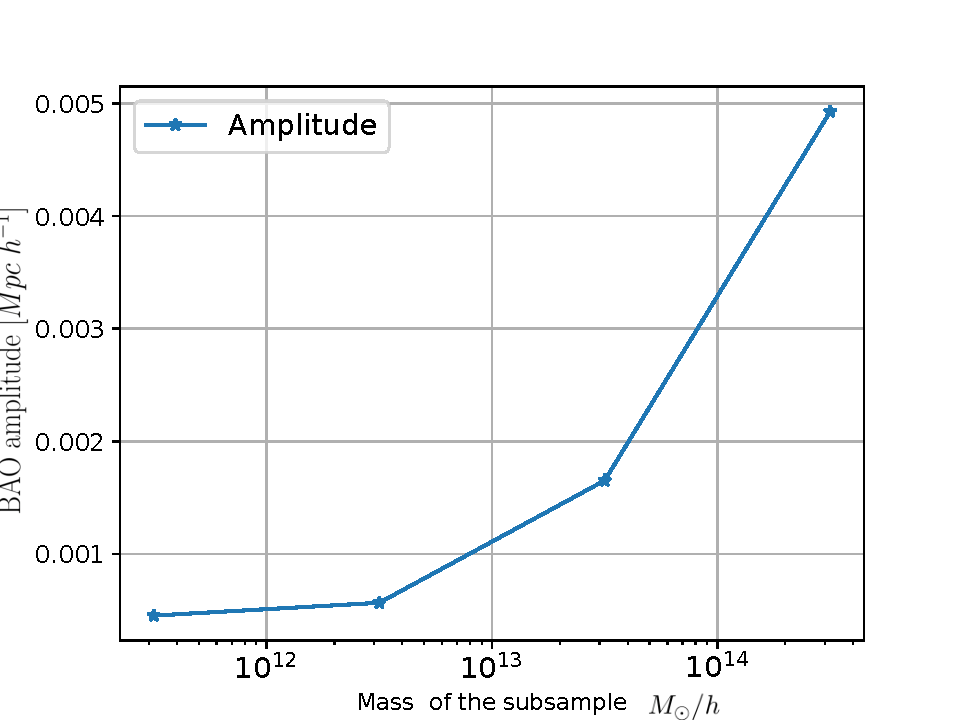
\includegraphics[width=0.8\textwidth]{Images/chapter4/Amp_vs_Mh.pdf}
       \caption{\small Amplitude of BAO for the populations obtained from MDPL simulation.}
       \label{ampl}
 \end{figure}
%**********************************************************************************************************************
%**********************************************************************************************************************
\begin{figure}[htbp]
       \centering
               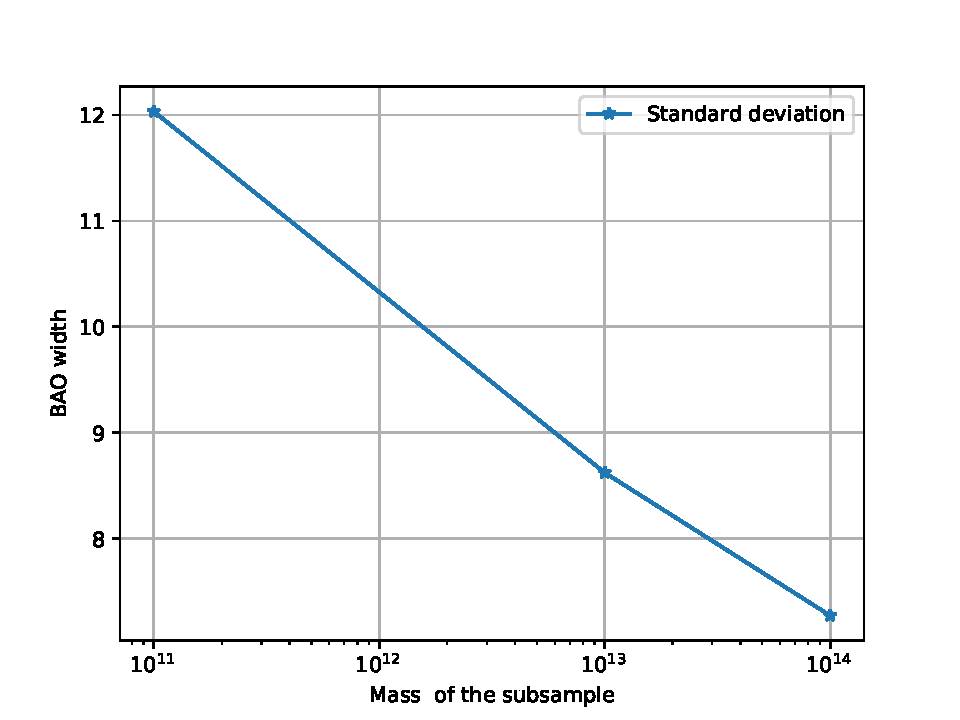
\includegraphics[width=0.8\textwidth]{Images/chapter4/Width_vs_Mh.pdf}
       \caption{\small Width of BAO for the populations obtained from MDPL simulation.}
       \label{width}
 \end{figure}
%**********************************************************************************************************************
%**********************************************************************************************************************
\begin{figure}[htbp]
       \centering
               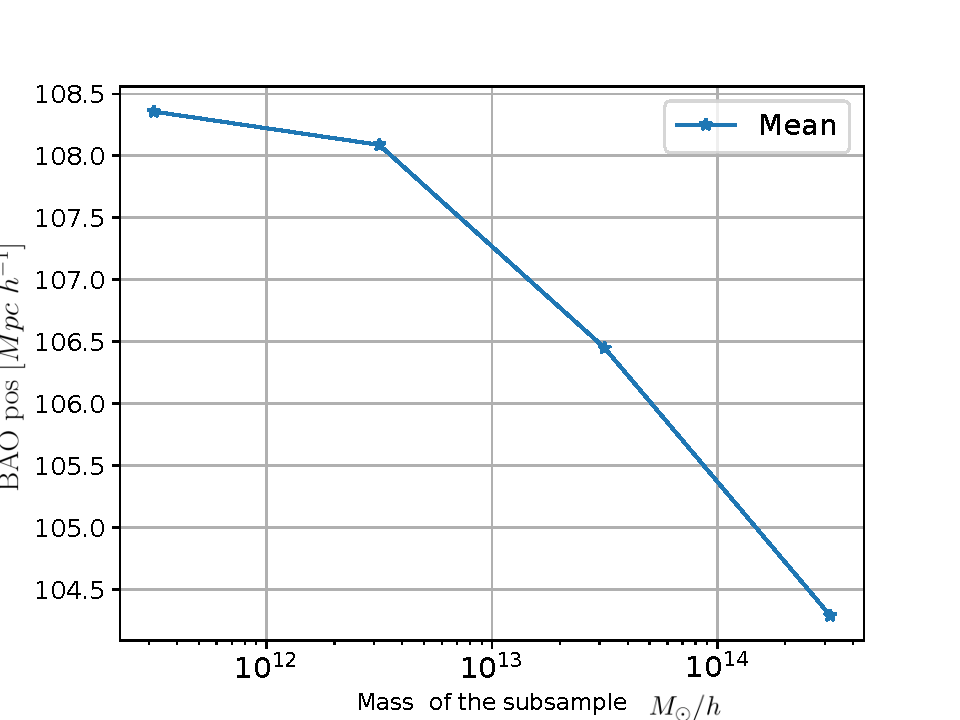
\includegraphics[width=0.8\textwidth]{Images/chapter4/Pos_vs_Mh.pdf}
       \caption{\small Position of BAO for the populations obtained from MDPL simulation.}
       \label{mean}
 \end{figure}
%**********************************************************************************************************************
\end{comment}